\documentclass{article}\usepackage[]{graphicx}\usepackage[dvipsnames]{xcolor}
% maxwidth is the original width if it is less than linewidth
% otherwise use linewidth (to make sure the graphics do not exceed the margin)
\makeatletter
\def\maxwidth{ %
  \ifdim\Gin@nat@width>\linewidth
    \linewidth
  \else
    \Gin@nat@width
  \fi
}
\makeatother

\definecolor{fgcolor}{rgb}{0.345, 0.345, 0.345}
\newcommand{\hlnum}[1]{\textcolor[rgb]{0.686,0.059,0.569}{#1}}%
\newcommand{\hlstr}[1]{\textcolor[rgb]{0.192,0.494,0.8}{#1}}%
\newcommand{\hlcom}[1]{\textcolor[rgb]{0.678,0.584,0.686}{\textit{#1}}}%
\newcommand{\hlopt}[1]{\textcolor[rgb]{0,0,0}{#1}}%
\newcommand{\hlstd}[1]{\textcolor[rgb]{0.345,0.345,0.345}{#1}}%
\newcommand{\hlkwa}[1]{\textcolor[rgb]{0.161,0.373,0.58}{\textbf{#1}}}%
\newcommand{\hlkwb}[1]{\textcolor[rgb]{0.69,0.353,0.396}{#1}}%
\newcommand{\hlkwc}[1]{\textcolor[rgb]{0.333,0.667,0.333}{#1}}%
\newcommand{\hlkwd}[1]{\textcolor[rgb]{0.737,0.353,0.396}{\textbf{#1}}}%
\let\hlipl\hlkwb

\usepackage{framed}
\makeatletter
\newenvironment{kframe}{%
 \def\at@end@of@kframe{}%
 \ifinner\ifhmode%
  \def\at@end@of@kframe{\end{minipage}}%
  \begin{minipage}{\columnwidth}%
 \fi\fi%
 \def\FrameCommand##1{\hskip\@totalleftmargin \hskip-\fboxsep
 \colorbox{shadecolor}{##1}\hskip-\fboxsep
     % There is no \\@totalrightmargin, so:
     \hskip-\linewidth \hskip-\@totalleftmargin \hskip\columnwidth}%
 \MakeFramed {\advance\hsize-\width
   \@totalleftmargin\z@ \linewidth\hsize
   \@setminipage}}%
 {\par\unskip\endMakeFramed%
 \at@end@of@kframe}
\makeatother

\definecolor{shadecolor}{rgb}{.97, .97, .97}
\definecolor{messagecolor}{rgb}{0, 0, 0}
\definecolor{warningcolor}{rgb}{1, 0, 1}
\definecolor{errorcolor}{rgb}{1, 0, 0}
\newenvironment{knitrout}{}{} % an empty environment to be redefined in TeX

\usepackage{alltt}
\usepackage{graphicx}
\usepackage{natbib}
\PassOptionsToPackage{hyphens}{url}\usepackage{hyperref}
\hypersetup{
    colorlinks=true,
    linkcolor=red,
    filecolor=magenta,
    urlcolor=purple,
    citecolor=violet
}


\usepackage[dvipsnames]{xcolor}
\colorlet{LightRubineRed}{RubineRed!100}
\definecolor{mypink2}{RGB}{219, 48, 122}

\title{Guide 1: Obtaining State Weather Station Data}
\author{Marc Los Huertos}
\date{\today~(ver. 0.97)}
\IfFileExists{upquote.sty}{\usepackage{upquote}}{}
\begin{document}
\maketitle

\section{Introduction}

\subsection{Goals}

Using a list of active weather stations in the United States, you  will download the data from five stations and write weather station data csv files. 

\subsection{Selected History of Climate Science}

Geologists have known the climate has been changing over the Earth's history. But what causes these changes has been a major research area for over 100 years. There are numerous drivers that contribute to changing climates -- including the arrangement of the continents on the planet, the distance to the sun, energy generated by the sun, volanic activity, and the composition of the Earth's atmosphere. 

It's the last one that we'll spend time because the Earth's temperature are changing pretty dramatically over the last 100 years and the cause is no mystery -- the human activity that has released carbon dioxide (CO$_2$) into the atmosphere. The two main sources of CO$_2$ is from land use change, e.g. deforestration, and the burning of fossil fuels, e.g. coal, oil, and natural gas. 

The first person to propose the role of CO$_2$ on the Earth's atmosphere was a Swedish scientist Svante Arrhenius, who figured out that CO$_2$ absorbs infarred light \citep{rodhe1997svante}. Moreover, he deduced that the Earth's temperature was actually warmer than it might otherwise be if CO$_2$ was not part of the Earth's atmosphere. 

\subsection{Why Look at Individual Stations?}

I don't think there is a single, perfect way to analyze and communicate climate change. But the beauty of the network of stations in the USA and around the world is that these stations record weather as expecienced by local people. And while indiviudual stations may not represent the overall regional and global patterns well, this give us a mechanism to connect local experiences to regional or global processes. 

Of course, some may fixate on the local pattern and remain unconvinced of the larger context and for those folks, there may be better ways to communicated climate data. 

However, I would be remiss in failing to mention that some may fixate on local patterns and use these patterns to ignore or to dimiss the patterns in other regions. 

Finally, the impacts of climate change are highly specific to the region in question. Thus, once someone understands the impacts on climate change in their region, they my not be able to appreciate how differnet the climate impacts might affect other peoples, who maybe more vulneratble, around the globe. 

Thus, with these weaknesses in mind, I will pursue this project with an eye to address these other issues at later stages.

\subsection{Approach}

\subsubsection{NOAA Data Records}

The US National Oceanic and Atmospheric Administration (NOAA) maintains several sources of digital weather data from the USA and beyond. These data have been collected from stations around the country to support a wide range of human activities that include farming, aviation, shipping, and even armed conflict. 

At various times, these records have been used to evaluate long-term climate change with varying success. Without a doubt, these data are not perfect, but they remain that foundation of an effective adn professionally maintained environmental monitoring program that engenders integrity, even when facing budget cuts. 

I will use these data to select for a station with a long record for each state in the USA. Future projects might evaluate the record for stations around the world, but we will see about that. 

\subsubsection{R Programming Language}

R is an open source programming environment that has become one of the most popular tools for statisticians and data scientists. Capitalizing on the open source framework, a wide range of libraries or packages have been developed to facilitate data processing, analysis, and graphical displays. 

%For the project we'll use a few packages that need to be installed and loaded. Using the lower right panel, you can install the packages by clicking on the "Packages" tab and then "Install" and then type in the package name and click "Install".

\subsection{Revised Document Structure}

Based on some feedback in the last week, I have re-orgnaized the document with bullets of the steps and then the code. In the following sections, I'll descriptions about ``what the code does and why". But several folks see the text and get tuned out.

There are two weaknesses with this approach that I can see. First, if the code does not work, you will have a really hard time figuring out why, since you have no idea what the code is supposed to do. Second, if the code works, you will not really be learning any R coding. Just how to copy and paste.

I have created a bunch of functions, which can then be used to collect Let's try this and see how it works! 

\subsection{Preparing R for the Project}

I suggest you do the following to prepare: 

\begin{enumerate}
  \item Create a folder for the project, I suggest ``Regional\_Climate\_Trends''. Note that there are no spaces in the folder name. 
  \item Next create a new R markdown file to write your code. Name and save it in your project folder. (For details see Section~\ref{subsec:RMarkdown})
  \item Download the file oldest.activestation.csv from the Canvas page and upload it to the directory you created in the previous step.
  \item Download the file called Guide1functions.R from the Canvas page and upload it to the directory you created in the previous step. 
  \item Open the file in Rstudio and run the code, using the ``source'' action item near the top, right of the editor window.
\end{enumerate}

\section{R Functions for Getting Weather Station Data}

\subsection{Marc's Custom Functions: Guide1functions.R}



These functions are designed so you don't have to type all the code! But check to see if they work for you, because they can (apparently) break really easily. 

From the Canvas page, go to the \href{https://github.com/marclos/RTricks/blob/master/04_Regional_Climate_Trends/Guides/Guide1functions.R}{Guide1functions.R} code and download the file to your computer. Then upload the file to a directory in Rstudio. I suggest you create a project called ``Regional\_Climate\_Trends'' and then upload the file to that directory. Please note, avoid spaces in your directory names.

Open the file in Rstudio and run the code, using the ``source'' action item near the top, right of the editor pane (Figure~\ref{fig:source_code}).

\begin{figure}[h]
\centering
\includegraphics[width=1.0\textwidth]{figure/Guide1Source.png}
\caption{The "source" action item is located in the upper right of the editor window. This will run the entire code with all the functions into the R environment.}
\label{fig:source_code}
\end{figure}

The function have been written to the R Environment and you can close Guide1.functions.R file. We don't need any more. However, if you'd like to see the functions, I have been written out in this document. 

\subsection{Creating a Record of Your Commands}

Use the Rmd file to record your R code and comments. This will help you remember what you did and why. See MarcsTemplate.Rmd as a skeleton file. 

\subsection{Function Descriptions and Use}

The following functions are used to select the weather stations, download data, and write weather station data csv files.

\begin{description}

\item[Subset Inventory Data with my.state]  The inventory data is a list of all the weather stations in the USA, US Territories, and Canada. This function will subset the data to only include the stations in the state of interest.

\begin{center}
\textbf{Function: \textcolor{Plum}{readInventory.fun()}}
\end{center}

This function requires two parameters to be set: filename and my.state. See Section~\ref{subsec:readInventory} for more details.

I suggest you use file.choose() and assign filename.csv to the path and name of the csv file in your project directory.  

Example of how to use the function:

\begin{knitrout}
\definecolor{shadecolor}{rgb}{0.969, 0.969, 0.969}\color{fgcolor}\begin{kframe}
\begin{alltt}
\hlstd{my.state} \hlkwb{<-} \hlstr{"CA"}
\hlstd{filename.csv} \hlkwb{<-}
  \hlstr{"/home/mwl04747/RTricks/04_Regional_Climate_Trends/stations.active.oldest.csv"}
\hlstd{my.inventory} \hlkwb{<-} \hlkwd{readInventory.fun}\hlstd{(filename.csv, my.state)}
\end{alltt}
\end{kframe}
\end{knitrout}

Creates a dataframe called my.inventory that contains the inventory data for the state/territory of interest. You should see that in the R environment. Note: The filename is cut off because my path is too long!

\item[Download and Read Selected Weather Station Data into R] This function will download the weather station data from the NOAA website and read it into R.

\begin{center}
\textbf{Function: \textcolor{Plum}{downloadStations.fun()}}
\end{center}

This functions requires two parameters: data path and name of inventory dataframe (my.inventory). The data path is a folder that you can always get your station data from if you need it. For example, if you need to update the data, you can just download the data from the NOAA website and then read it into R. For more information on this function see Section~\ref{subsec:downloadStations}.

The path to your data folder will be different, I created a directory to separate my data by class year, you don't need that! But it is nice to keep the data in a separate folder so things don't get to hectic.

An example of how to use the function: 

\begin{knitrout}
\definecolor{shadecolor}{rgb}{0.969, 0.969, 0.969}\color{fgcolor}\begin{kframe}
\begin{alltt}
\hlstd{datapath} \hlkwb{=} \hlstr{"/home/mwl04747/RTricks/04_Regional_Climate_Trends/Data/SP24/"}
\hlkwd{downloadStations.fun}\hlstd{(datapath, my.inventory)}
\end{alltt}
\end{kframe}
\end{knitrout}

This will download the data from the NOAA website and read it into R then written as compresseed gz and uncompressed czv files in your data folder. Check to see that you have both csv.gz and .csv files in your data folder.

\end{description}

\noindent {\Large\textcolor{ForestGreen}{You're are done with this guide, go to Guide 2!}}

\section{Explaining the Process and Code}

\subsection{Working with a R Markdown File}\label{subsec:RMarkdown}

To record your history of R code, I suggest use an Rmarkdown file to keep your code handy. 

To do this open a new file and select R Markdown -- Define a title, author, and output format as PDF. Then save the file (Figure~\ref{fig:RMarkdown}). 

\begin{figure}[h]
\centering
\includegraphics[width=1.0\textwidth]{/home/mwl04747/RTricks/04_Regional_Climate_Trends/Guides/figure/Guide1NewRMarkdown.png}
\caption{Creating a new R Markdown file.}
\label{fig:RMarkdown}
\end{figure}


Then save the file in your project folder and knit the file to create a PDF. Look at the PDF to see how various parts of the Rmd file were knitted. Notice that there are generally two sections: text and R chunks. As you write th R code, you will can record your code in the R chunks AND develop the output into a document for future reference.

Look carefully at the Rmd file and take note of the following: First, there are chunks of R code separated from the text by a line of three backticks. Second, the R code is written in the chunks and the output is written below the code. Finally, there is a set of backticks at the end of the code chunk. This section is gray and is where you can record your Rcode. I suggest you delete existing the one line of R code inside the existing template chuck.  

\subsubsection{R Environment and knitr}

When you knit, R starts a new environment and runs the code in the chunks. But that means the new environment doesn't have the data you have created in your current environment. So, I suggest you use the R markdown to double check that everything is working well. 

I have created an R Markdown file for you to use. It is called MarcsTemplate.Rmd. As a template, you can use and change the code as you go. 

\subsection{Defining Path \& Read Data}

First, we install some packages and read in the data. I suggest you create a folder for the project (I created one called ``04\_Regional\_Climate\_Trends").  To get the working directory and filename, we can use the file.choose() function from the console:

\begin{verbatim}
> file.choose()
\end{verbatim}

Then paste the result in the Rmd file to track the results to define the file name:\footnote{I use a function here() from the ``here library'', but it's a bit tricky to use and you can use that if you prefer.}

\begin{knitrout}
\definecolor{shadecolor}{rgb}{0.969, 0.969, 0.969}\color{fgcolor}\begin{kframe}
\begin{alltt}
\hlstd{filename} \hlkwb{=} \hlstr{"home/mwl04747/RTricks/04_Regional_Climate_Trends/stations.active.oldest.csv"}


\hlcom{# OR what I use! see the footnote.}
\hlkwd{library}\hlstd{(here)}
\hlstd{filename} \hlkwb{=} \hlkwd{here}\hlstd{(}\hlstr{"04_Regional_Climate_Trends"}\hlstd{,} \hlstr{"stations.active.oldest.csv"}\hlstd{)}
\end{alltt}
\end{kframe}
\end{knitrout}

%suggest you change the name of the file to something more descriptive.

\subsection{Selecting Weather Records by State}

\subsubsection{Map US Weather Stations}

Here's a map of the weather stations in the dataset. Pretty lame map!  We'll make a better one later.\footnote{Evelyn/Brody: This is a good change to see how to use R for map making! First we need to transform that data.}

\begin{knitrout}
\definecolor{shadecolor}{rgb}{0.969, 0.969, 0.969}\color{fgcolor}\begin{kframe}
\begin{alltt}
\hlstd{stations.active.oldest} \hlkwb{=}
  \hlkwd{read.csv}\hlstd{(}\hlkwd{paste0}\hlstd{(}\hlkwd{here}\hlstd{(),} \hlstr{"/04_Regional_Climate_Trends/"}\hlstd{,}
                  \hlstr{"stations.active.oldest.csv"}\hlstd{))}
\hlkwd{plot}\hlstd{(stations.active.oldest}\hlopt{$}\hlstd{LONGITUDE,}
     \hlstd{stations.active.oldest}\hlopt{$}\hlstd{LATITUDE,}
     \hlkwc{xlab} \hlstd{=} \hlstr{"Longitude"}\hlstd{,}\hlkwc{ylab} \hlstd{=} \hlstr{"Latitude"}\hlstd{,}
     \hlkwc{pch}\hlstd{=}\hlnum{20}\hlstd{,} \hlkwc{cex}\hlstd{=}\hlnum{0.2}\hlstd{,} \hlkwc{col}\hlstd{=}\hlstr{'gray40'}\hlstd{,} \hlkwc{las}\hlstd{=}\hlnum{1}\hlstd{,}
     \hlkwc{main} \hlstd{=} \hlstr{"US Weather Stations"}\hlstd{)}
\end{alltt}
\end{kframe}
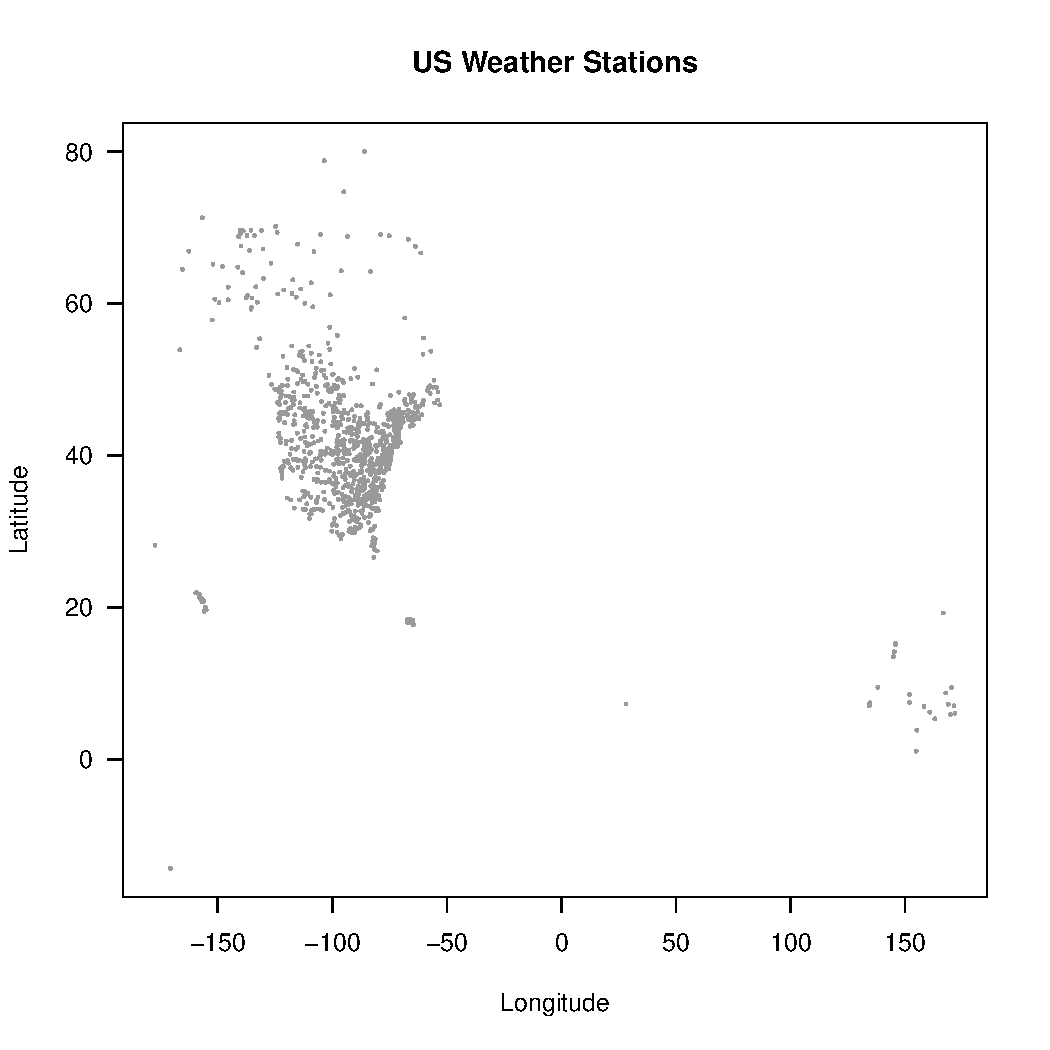
\includegraphics[width=\maxwidth]{figure/unnamed-chunk-4-1} 
\end{knitrout}

There are numerous ways to analyze temperature records, where stations can be analyzed individually or records could be sampled and analyzed in spatially in grids. Each of these are valid approaches depending on the question to be addressed. 

Here are the questions we will address: 

\begin{itemize}
  \item What stations have the longest meteorological records in the USA?
  \item Can we determine the reliability of these stations?
  \item Finally, is there a temperature trend?
\end{itemize}

\subsection{Subset Station Inventory by State}

This uses the stations.active.oldest file to download the data from the NOAA website based on the state you have choose.

The URL for a description of the data is: \url{https://www.ncdc.noaa.gov/cdo-web/datasets/GHCND/stations/GHCND:USW00023230/detail}.

\section{Function Details}

\subsection{readInventory.fun}\label{subsec:readInventory}

This function...

Here's the function:

\begin{knitrout}
\definecolor{shadecolor}{rgb}{0.969, 0.969, 0.969}\color{fgcolor}\begin{kframe}
\begin{verbatim}
## function (filename, my.state) 
## {
##     inventory.active.oldest <- read.csv(filename)
##     my.inventory = subset(inventory.active.oldest, STATE == my.state)
##     return(my.inventory)
## }
\end{verbatim}
\end{kframe}
\end{knitrout}

\subsection{downloadStations.fun}\label{subsec:downloadStations}\section{Download Data from NOAA}





Here's the function:

\begin{knitrout}
\definecolor{shadecolor}{rgb}{0.969, 0.969, 0.969}\color{fgcolor}\begin{kframe}
\begin{verbatim}
## function (datafolder, my.inventory = my.inventory) 
## {
##     colnames <- c("ID", "DATE", "ELEMENT", "VALUE", "M-FLAG", 
##         "Q-FLAG", "S-FLAG", "OBS-TIME")
##     for (i in 1:nrow(my.inventory)) {
##         url = paste0("https://www.ncei.noaa.gov/pub/data/ghcn/daily/by_station/", 
##             my.inventory$ID[i], ".csv.gz")
##         download.file(url, paste0(datafolder, my.inventory$ID[i], 
##             ".csv.gz"), quiet = FALSE, mode = "w", cacheOK = TRUE)
##         station.temp <- read.csv(paste0(datafolder, my.inventory$ID[i], 
##             ".csv.gz"), header = FALSE)
##         names(station.temp) <- colnames
##         filename = paste0(datafolder, my.inventory$ID[i], ".csv")
##         write.csv(station.temp, filename, row.names = FALSE)
##         print(paste("Index (Loop) ", i, " Completed."))
##         print("NOAA site can stall -- if the loop errors out, try again.")
##     }
##     print("Think about something you are grateful for today!")
##     write.csv(my.inventory, paste0(datafolder, "my.inventory.csv"), 
##         row.names = FALSE)
## }
## <bytecode: 0x297d9e0>
\end{verbatim}
\end{kframe}
\end{knitrout}

\section{Trouble Shooting and Workarounds}

I will be getting all the guides working before working on this! But if there are errors with the custom function, this is where workarounds will be described! Please Slack me and mentors if you have any problems!

\subsection{NA.csv as a duplicate?}

I am not sure why, but in the downloadStations.fun(), the file is saved as NA.csv. I have no idea why. If you find this, let me know, I'd like to figure out if their is a bug in the code creating this csv.
If you find a NA.csv in your folder, please let marc or mentors know and we will try to figure out what is going on.

\subsection{Download gz files with folder concantentated names}

Five students had this issue on Wednesday, but no one on Tuesday. That less than half the students had this issue is perplexing and I figured out that some students were using old functions, so I updated the functions and changed the Guide fuction file to reflect this change. 

\section{rNOAA -- Unsupported and Deprecated Library}

The rNOAA package has been deprecated, so all the 2000-2022 code is no longer working. I have commented out the text -- but should I need to re-run the code, I have some of the description in the Rmd file. 

%\subsubsection{Identify List of State IDs (FIPS)}

%Using the rNOAA library in R, we can query NOAA's database to identify station codes (FIPS) by state. With the states and some territories, there are 55 FIPS for US weather stations. Althogh these include the District of Columbia, they do not include US Territories, sich as Guam, Puerto Rico, Marshall Islands, etc. We'll have to use a different search code for these.

%rNOAA has a simple function to list for each of the states and the weather stations in each. I use ncdc\_locs() functions to select each state and ncdc\_station() to obtain the station ids with the longest records. 

%The function queries the NOAA website and retrieves state codes, ``FIPS:XX''. Each state has a number of weather stations,\footnote{Project Idea: It would be nice to make a map of how concentrated the stations spatially.} some with a long record, some with a short record, and some with numerous interruptions. Our goal is to select a long record with few missing data. 

%\subsubsection{Selection Stations}

%With the state ids, we can evaluate the metadata for all the weather stations, which will work to get the longest records, using \texttt{ncdc\_stations()}. 

%First, we subset the data for stations that actively collecting data. Then we'll sort to the active stations to find the one with the longest records. We will use these stations for our analysis. 

%There were some records that didn't have robust TMAX/TMIN records, so there are some states that I had to manually select an alternative stations. 



% bibiliography section here-------------------------------------------
%\clearpage

\bibliographystyle{apalike}
%\renewcommand\bibname{References}{}
\bibliography{/home/mwl04747/RTricks/references}%	\addcontentsline{toc}{chapter}{References}


\end{document}
